\section{Обзор}
Предлагаемый в данной работе алгоритм заимствует распространённые принципы существующих работ данной области. Помимо этого переиспользуется RNGLR-алгоритм синтаксического анализа вместе с соответствующими структурами данных. В данном разделе приведён обзор подходов к анализу встроенных языков, дано краткое описание RNGLR-алгоритма, а также описан проект, в рамках которого велась разработка предложенного алгоритма.

Задача анализа динамически формируемых выражений актуальна как с точки зрения обеспечения безопасности программного обеспечения (поиск мест, уязвимых для SQL-инъекций), так и для разработки, сопровождения и модернизации систем, разработанных с применением встроенных языков. Для решения этих задач существует ряд основанных на них подходов и инструментов, которые будут описаны ниже.
Проверка включения языков. Строится язык L1 —  некоторое приближение языка L, генерируемого программой, и проверяется его включение в язык, описанный эталонной грамматикой L2. Основной недостаток данного подхода — невозможность получить какую-либо информацию, кроме знания о вхождении или не вхождении одного языка в другой. Как следствие, проведение более сложных видов статического анализа или трансформации невозможно. Можно выделить несколько вариантов данного подхода, различающихся классом языка L1.
Регулярная аппроксимация: L1 является регулярным языком. Однако язык L не обязан быть регулярным, так как его генератор может быть реализован на тьюринг-полном языке, что может приводить к существенной потере точности при построении приближения. Достоинством такого подхода является разрешимость задачи проверки включения L1 в L2 для регулярного L1 и L2, принадлежащего некоторым подклассам КС языков, таким как детерминированные или LL(k) []. Инструмент, реализующий данный подход —  Java String Analizer [], являющийся анализатором строковых выражений в коде на Java.
Контекстно-свободное приближение: L1 является контекстно-свободным языком.  Достоинством является то, что такое приближение более точное, однако проверка включения для двух КС языков является неразрешимой задачей []. По  этой причине в результате будет получено неточное решение. Данный подход реализован в инструменте PHPSA [], предназначенном для проверки корректности динамически формируемых программами на PHP выражений.
Синтаксический анализ. Основан на применении техник синтаксического анализа для работы с динамически формируемыми выражениями. Благодаря этому, кроме проверки корректности выражений становится возможным решение более сложных задач, требующих знаний о структуре вывода или работы с деревом разбора, таких как семантический анализ или трансформации. Ниже перечислены существующие на текущий момент варианты данного подхода.
Абстрактный LR-анализ. В исследованиях группы во главе  с Kyung-Goo Doh предлагается комбинация анализа потока данных и синтаксического анализа на основе LALR(k) алгоритма, позволяющая строить множество LR-стеков для всех значений строкового выражения [,]. Так как задача проверки включения для двух КС языков неразрешима, то решение приближённое. В работе [] обоснована возможность семантического анализа на основе классического для LR-анализа механизма: атрибутных грамматик [Дракон] и выполнения семантического действия при выполнении свёртки. Однако не до конца исследована эффективность данного подхода при работе с семантическими действиями, требующими больших ресурсов при вычислении.
Синтаксический анализ регулярного множества. Для языка L строится регулярная аппроксимация. Далее над построенной аппроксимацией решаются задачи лексического и синтаксического анализа. Данный подход рассмотрен в работе [] и реализован в инструменте Alvor. Данный инструмент является плагином к среде разработки Eclipse, предоставляющим поддержку встроенного SQL в Java: статический поиск ошибок, тестирование запросов в базе данных. Использование атрибутных грамматик — классического для LR-анализа способа задания семантики — и построение леса разбора в рамках данного подхода также не обсуждается.

\subsection{Регулярная аппроксимация множества значений динамически формируемых выражений}
Программа, использующая встроенные текстовые языки, является программой-генератором: она может порождать некоторое множество предложений и определяет некоторый язык L. 
Многие практически значимые задачи, связанные с динамически формируемыми выражениями, среди которых самая активно исследуемая — проверка корректности генерируемых предложений, связаны с 
проверкой включения языка L в некоторый другой язык L2. Как правило, язык L2 является некоторым языком программирования, выражения на котором должна генерировать программа (SQL, HTML). 
Язык L2 часто является КС языком. Однако проверка включения для двух КС языков неразрешима, но проверка включения регулярного языка в некоторые практически значимые подклассы КС языков (LL(k), 
детерминированные КС) разрешима. По этой причине в ряде работ [,], посвящённых анализу динамически формируемых выражений, используется регулярное приближение языка L. Важно, что можно построить 
регулярный язык, являющийся приближением сверху для языка L[], то есть аппроксимацию сверху (over-approximation): регулярный язык содержит все предложения, генерируемые программой и, возможно, ещё какие-то. 
Благодаря этому можно говорить о достоверности многих видов статического анализа, например поиска ошибок, в том смысле, что если алгоритм анализа регулярной аппроксимации не сообщил о наличии ошибок, 
то все выражения языка L корректны. Однако, могут быть ложные срабатывания: ошибочное предложение может принадлежать аппроксимации, но не принадлежать языку L.

Таким образом, регулярная аппроксимация для множества значений динамически формируемых выражений позволяет решать многие важные задачи. На практике для её представления можно использовать конечные автоматы, 
так как для любого регулярного языка L можно построить конечный автомат, такой что он принимает те и только те цепочки, которые принадлежат языку L. В данной работе используется регулярная аппроксимация 
множества значений строковых выражений, представленная в виде конечного автомата.

\subsection{RNGLR-алгоритм}
RNGLR-алгоритм (Right-Nulled Generalized LR) является модификацией предложенного Масару Томитой алгоритма Generalized LR (GLR)~\cite{Tomita}, предназначенного для анализа естественных языков. 
GLR-алгоритм был предназначен для анализа неоднозначных контекстно-свободных грамматик. В процессе работы с такими грамматиками не всегда на основе имеющейся информации можно однозначно принять решение 
о следующем шаге: выполнить чтение очередного токена или выполнить свёртку (Shift/Reduce конфликт); по какому из правил выполнять свёртку(Reduce/Reduce конфликт). Это приводит к тому, что для одной 
входной цепочки можно получить несколько вариантов разбора и, соответственно, несколько LR-стеков.  

Оригинальный алгоритм, предложенный Томитой, не был способен анализировать все контекстно-свободные грамматики. 
Элизабет Скотт и Адриан Джонстоун предложили RNGLR-алгоритм, который расширяет GLR-алгоритм специальным способом обработки обнуляемых справа 
правил (right-nullable rules, имеющих вид $\mathrm{A} \rightarrow \alpha \beta$, где $\beta$ выводит пустую строку $\varepsilon$).

\begin{listing}[!ht]
\begin{algorithmic}[1]
\caption{RNGLR-алгоритм}
\label{rnglr}
\Function{parse}{$grammar, input$}
  \State{$\mathcal{R} \gets \emptyset$} \Comment{Очередь троек: вершина GSS, нетерминал, длина свёртки}
  \State{$\mathcal{Q} \gets \emptyset$} \Comment{Коллекция пар: вершина GSS, состояние парсера}
  \If{$input = \varepsilon$}
    \If{$grammar$ accepts empty input} {report success}
    \Else { report failure}
    \EndIf
  \Else
    \State{\Call{addVertex}{$0, 0, startState$}}
    \ForAll{$i$ in $0..input.Length-1$}
      \State{\Call{reduce}{$i$}}
      \State{\Call{push}{$i$}}
    \EndFor
    \If{$i=input.Length-1$ and there is a vertex in the last level of GSS which state is accepting}
      \State{report success}
    \Else { report failure}
    \EndIf
  \EndIf
\EndFunction
\Function{reduce}{$i$}
  \While{$\mathcal{R}$ is not empty}
    \State{$(v, N, l) \gets \mathcal{R}.Dequeue()$}
    \State{find the set $\mathcal{X}$ of vertices reachable from $v$ along the path of length $(l-1)$}
    \State{or length $0$ if $l=0$}
    \ForAll{$v_{h} = (level_{h}, state_{h})$ in $\mathcal{X}$}
      \State{$state_{t} \gets$ calculate new state by $state_{h}$ and nonterminal $N$}
      \State{\Call{addEdge}{$i, v_{h}, v.level, state_{tail}, (l=0)$}}
    \EndFor
  \EndWhile
\EndFunction
\Function{push}{$i$}
  \State{$\mathcal{Q^{'}} \gets$ copy $\mathcal{Q}$}
  \While{$\mathcal{Q^{'}}$ is not empty}
    \State{$(v, state) \gets \mathcal{Q}.Dequeue()$}
    \State{\Call{addEdge}{$i, v, v.level + 1, state, false$}}
  \EndWhile
\EndFunction
\end{algorithmic}
\end{listing}

\begin{listing}[!ht]
\begin{algorithmic}[1]
\caption{Построение GSS}
\label{RNGLRMain}
\Function{addVertex}{$i, level, state$}
  \If{GSS does not contain vertex $v = (level, state)$}
    \State{add new vertex $v = (level, state)$ to GSS}
    \State{calculate the set of shifts by $v$ and the $input[i+1]$ and add them to $\mathcal{Q}$}
    \State{calculate the set of zero-reductions by $v$ and the $input[i+1]$ and}
    \State{add them to $\mathcal{R}$}
  \EndIf
  \State{\Return{$v$}}
\EndFunction
\Function{addEdge}{$i, v_{h}, level_{t}, state_{t}, isZeroReduction$}
  \State{$v_{t} \gets$ \Call{addVertex}{$i, level_{t}, state_{t}$}}
  \If{GSS does not contain edge from $v_{t}$ to $v_{h}$}
    \State{add new edge from $v_{t}$ to $v_{h}$ to GSS}
    \If{not $isZeroReduction$}
      \State{calculate the set of reductions by $v$ and the $input[i+1]$ and}
      \State{add them to $\mathcal{R}$}
    \EndIf
  \EndIf
\EndFunction
\end{algorithmic}
\end{listing}

Для эффективного представления множества стеков во время синтаксического анализа в алгоритме RNGLR используется структурированный в виде графа стек (Graph Structured Stack, GSS), который является ориентированным графом, чьи вершины соответствуют  элементам отдельных стеков, а ребра связывают последовательные элементы. Каждая вершина может иметь несколько входящих рёбер, что соответствует слиянию нескольких стеков, за счёт чего производится переиспользование общих участков отдельных стеков. Вершина GSS~--- это пара $(s,l)$, где $s$~--- состояние парсера, а $l$~--- уровень (позиция во входном потоке).

RNGLR-алгоритм последовательно считывает символы входного потока слева направо, по одному за раз, и строит GSS по "слоям": сначала осуществляются все возможные свёртки для данного символа, после чего сдвигается следующий символ со входа. Свёртка или сдвиг модифицируют GSS следующим образом. Предположим, что необходимо добавить ребро $(v_t,v_h)$ в GSS. По построению, конечная вершина добавляемой дуги к такому моменту уже обязательно находится в GSS. Если начальная вершина также содержится в GSS, то в граф добавляется новое ребро (если оно ранее не было добавлено), иначе создаются и добавляются в граф и начальная вершина, и ребро. Каждый раз, когда создаётся новая вершина $v=(s,l)$, алгоритм вычисляет новое состояние парсера $s'$ по $s$ и следующему символу входного потока. Пара $(v,s')$, называемая push, добавляется в глобальную коллекцию $\mathcal{Q}$. Также при добавлении новой вершины в GSS вычисляется множество $\varepsilon$-свёрток, после чего элементы этого множества добавляются в глобальную очередь $\mathcal{R}$. Свёртки длины $l>0$ вычисляются и добавляются в $\mathcal{R}$ каждый раз, когда создаётся новое (не-$\varepsilon$) ребро. Подробное описание работы со структурированным в виде графа стеком GSS содержится в алгоритме~\ref{RNGLRMain}.

В силу неоднозначности грамматики входная строка может иметь несколько деревьев вывода, как правило, содержащих множество идентичных поддреревьев. Для того, чтобы компактно хранить множество деревьев вывода, 
используется компактное представление леса разбора (Shared Packed Parse Forest, SPPF)~\cite{SPPF}, предложенное Rekers []. В общем случае SPPF может быть произвольным связанным графом, однако из него всегда можно 
восстановить те и только те деревья, которые соответствуют какому либо варианту разбора данной входной цепочки. Это достигается благодаря тому, что в SPPF кроме вершин, соответствующих 
непосредственно узлам синтаксического дерева, могут присутствовать специальные типы вершин, отвечающие за корректное переиспользование поддеревьев. Структура SPPF описана ниже.
\begin{enumerate}
  \item \emph{Корень} (то есть, вершина, не имеющая входящих дуг) соответствует стартовому нетерминалу грамматики.
  \item \emph{Терминальные} вершины, не имеющие исходящих дуг, соответствуют либо терминалам грамматики, либо деревьям вывода пустой строки $\varepsilon$.
  \item \emph{Нетерминальные} вершины являются корнем дерева вывода некоторого нетерминала грамматики; только вершины-продукции могут быть непосредственно достижимы из таких вершин.
  \item \emph{Вершины-продукции}, представляющие правую часть правила грамматики для соответствующего нетерминала. Вершины, непосредственно достижимые из них, упорядочены и могут являться либо терминальными, либо нетерминальными вершинами. Количество таких вершин лежит в промежутке $[l-k..l]$, где $l$~--- это длина правой части продукции, а $k$~--- количество финальных символов, выводящих $\varepsilon$ (правые обнуляемые символы игнорируются для уменьшения потребления памяти).
\end{enumerate}

SPPF создаётся одновременно с построением GSS. Каждое ребро GSS ассоциировано с либо с терминальным, либо с нетерминальным узлом. Когда добавление ребра в GSS происходит во время операции push, новая терминальная вершина создаётся и ассоциируется с ребром. Нетерминальные вершины ассоциируются с ребрами, добавленными во время операции reduce. Если ребро уже было в GSS, к ассоциированной с ним нетерминальной вершине добавляется новая вершина-продукция. Подграфы, ассоциированные с рёбрами пути, вдоль которого осуществлялась свёртка, добавляются как дети к вершине-продукции. После того, как входной поток прочитан до конца, производится поиск всех вершин, имеющих принимающее состояние анализатора, после чего подграфы, ассоциированные с исходящими из таких вершин рёбрами, объединяются в один граф. Из полученного графа удаляются все недостижимые из корня вершины, что в итоге оставляет только корректные деревья разбора для входной строки. 

Листинг~\ref{rnglr} представляет более детальное описание алгоритма.

\subsection{Проект YaccConstructor и платформа для анализа встроенных языков}
В рамках проекта YaccConstructor~\cite{YC} лаборатории языков инструментов JetBrains на математико-механическом факультете СПбГУ проводятся исследования в области лексического и синтаксического анализа, 
а также статического анализа встроенных языков. Проект YaccConstructor представляет собой модульный инструмент, имеет собственный язык спецификации грамматик, объединяет различные алгоритмы лексического и 
синтаксического анализа. В рамках проекта была создана платформа для статического анализа встроенного кода~\cite{SECR14}; диаграмма последовательности, иллюстрирующая взаимодействие модулей платформы 
представлена на рисунке~\ref{seq}. Цветом выделена компонента, осуществляющая синтаксический анализ множества значений динамически формируемого выражения. 
\begin{figure}[!h]
 \centering
 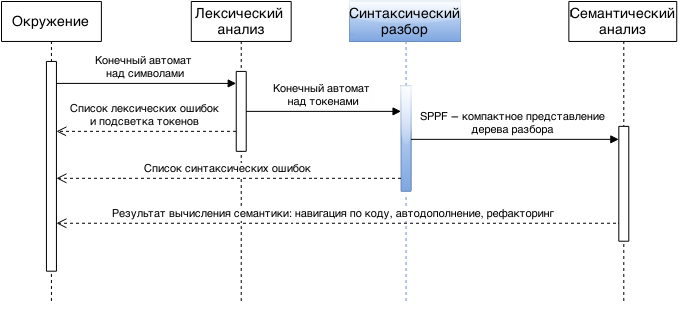
\includegraphics[width=15cm]{pics/Seq_rus.png}
 \caption{Диаграмма последовательности: взаимодействие компонентов
инструмента YaccConstructor}
 \label{seq}
\end{figure}

Предыдущая реализация платформы работала с грубой аппроксимацией, которая не осуществляла поддержку формирования выражения в циклах и с помощью строковых выражений~\cite{SECR13}. Используемая аппроксимация не являлась аппроксимацией сверху, что сказывалось на точности результатов анализа, и поэтому впоследствии она была заменена на регулярную. Однако это повлекло необходимость изменения алгоритма синтаксического анализа, чему и посвящена данная работа. 